\documentclass[aspectratio=169,11pt]{beamer}

% TEMA Y COLORES
\usetheme{Madrid}
\usecolortheme{whale}

\definecolor{primaryblue}{RGB}{0,102,153}
\definecolor{accentgreen}{RGB}{0,128,0}
\definecolor{accentorange}{RGB}{204,102,0}
\definecolor{darkgray}{RGB}{64,64,64}

\setbeamercolor{palette primary}{bg=primaryblue,fg=white}
\setbeamercolor{palette secondary}{bg=primaryblue!80,fg=white}
\setbeamercolor{palette tertiary}{bg=primaryblue!60,fg=white}
\setbeamercolor{structure}{fg=primaryblue}
\setbeamercolor{block title}{bg=primaryblue,fg=white}
\setbeamercolor{block body}{bg=primaryblue!10}
\setbeamercolor{block title example}{bg=accentgreen,fg=white}
\setbeamercolor{block body example}{bg=accentgreen!10}
\setbeamercolor{block title alerted}{bg=accentorange,fg=white}
\setbeamercolor{block body alerted}{bg=accentorange!10}

% PAQUETES
\usepackage[utf8]{inputenc}
\usepackage[T1]{fontenc}
\usepackage{amsmath,amssymb}
\usepackage{booktabs}
\usepackage{tikz}
\usepackage{pgfplots}
\usepackage{listings}
\usepackage{multicol}

\pgfplotsset{compat=1.17}

% CÓDIGO PYTHON
\lstdefinestyle{pythonstyle}{
    language=Python,
    basicstyle=\ttfamily\footnotesize,
    keywordstyle=\color{blue}\bfseries,
    stringstyle=\color{red},
    commentstyle=\color{accentgreen}\itshape,
    frame=single,
    breaklines=true,
    showstringspaces=false,
    backgroundcolor=\color{gray!10}
}

% NAVEGACIÓN Y PIE DE PÁGINA
\setbeamertemplate{navigation symbols}{}
\setbeamertemplate{footline}{
    \leavevmode%
    \hbox{%
        \begin{beamercolorbox}[wd=.333333\paperwidth,ht=2.25ex,dp=1ex,center]{author in head/foot}%
            \usebeamerfont{author in head/foot}Matemáticas Financieras
        \end{beamercolorbox}%
        \begin{beamercolorbox}[wd=.333333\paperwidth,ht=2.25ex,dp=1ex,center]{title in head/foot}%
            \usebeamerfont{title in head/foot}Sesión 8
        \end{beamercolorbox}%
        \begin{beamercolorbox}[wd=.333333\paperwidth,ht=2.25ex,dp=1ex,right]{date in head/foot}%
            \usebeamerfont{date in head/foot}\insertframenumber{} / \inserttotalframenumber\hspace*{2ex}
        \end{beamercolorbox}}%
    \vskip0pt%
}

\title[Sesión 8]{Valuación de Bonos}
\subtitle{Precio, rendimiento y curvas de tasas}
\author{Matemáticas Financieras}
\institute{Valor del Dinero en el Tiempo}
\date{Semana 4 | Clase 2 | Duración: 1h 50min}

\begin{document}

% ===========================================
% SECCIÓN 1: PORTADA Y CONTENIDO
% ===========================================

\begin{frame}
    \titlepage
\end{frame}

\begin{frame}{Contenido de la Sesión}
    \tableofcontents
\end{frame}

% ===========================================
% SECCIÓN 2: INTRODUCCIÓN
% ===========================================
\section{Introducción}

\begin{frame}{Conexión con la Sesión Anterior}
    \begin{block}{Sesión 7: Amortización de Préstamos}
        Vimos cómo se estructuran los préstamos bancarios (deuda privada):
        \begin{itemize}
            \item Sistema francés, alemán, americano
            \item Tablas de amortización
        \end{itemize}
    \end{block}

    \pause
    \vspace{0.3cm}

    \begin{alertblock}{Hoy: Bonos (Deuda Pública Negociable)}
        Los bonos son instrumentos de deuda que:
        \begin{itemize}
            \item Se negocian en mercados secundarios
            \item Tienen un precio que fluctúa
            \item Pagan cupones periódicos (generalmente)
            \item Devuelven el principal al vencimiento
        \end{itemize}
    \end{alertblock}
\end{frame}

\begin{frame}{Objetivos de Aprendizaje}
    Al finalizar esta sesión, serás capaz de:
    \begin{enumerate}
        \item Identificar los componentes de un bono
        \item Calcular el precio de un bono dada una tasa de descuento
        \item Calcular el rendimiento al vencimiento (YTM)
        \item Entender la relación inversa precio-rendimiento
        \item Interpretar la curva de rendimientos
        \item Aplicar interpolación lineal de tasas
        \item Clasificar bonos como prima, par o descuento
    \end{enumerate}
\end{frame}

\begin{frame}{Anatomía de un Bono}
    \begin{block}{Componentes Principales}
        \begin{itemize}
            \item \textbf{Valor Nominal / Par ($F$):} Monto que se paga al vencimiento (típicamente \$1,000)
            \item \textbf{Tasa Cupón ($c$):} Tasa anual sobre el valor nominal
            \item \textbf{Cupón ($C$):} Pago periódico = $F \times c / m$ (donde $m$ = pagos por año)
            \item \textbf{Vencimiento ($n$):} Fecha de pago del principal
            \item \textbf{Precio ($P$):} Valor de mercado del bono
        \end{itemize}
    \end{block}

    \pause
    \vspace{0.3cm}

    \begin{exampleblock}{Ejemplo}
        Bono del Tesoro: \$1,000 nominal, cupón 5\% semestral, 10 años.

        Cupón = $1,000 \times 0.05 / 2 = \$25$ cada 6 meses.

        20 pagos de \$25 + \$1,000 al final.
    \end{exampleblock}
\end{frame}

% ===========================================
% SECCIÓN 3: PRECIO DE UN BONO
% ===========================================
\section{Valuación de Bonos}

\begin{frame}{Diagrama de Flujos de un Bono}
    \begin{center}
        \begin{tikzpicture}[scale=0.85]
            % Línea de tiempo
            \draw[thick, ->] (-0.5,0) -- (12,0) node[right] {$t$};

            % Marcas
            \foreach \x/\label in {0/0, 2/1, 4/2, 6/3, 10/n} {
                \draw (\x,0.1) -- (\x,-0.1) node[below] {\label};
            }
            \node at (8,0) {$\cdots$};

            % Cupones
            \foreach \x in {2, 4, 6, 10} {
                \draw[thick, ->, accentgreen] (\x,0) -- (\x,1.0);
            }
            \node[accentgreen, above] at (2,1.1) {$C$};
            \node[accentgreen, above] at (4,1.1) {$C$};
            \node[accentgreen, above] at (6,1.1) {$C$};
            \node[accentgreen, above] at (10,1.1) {$C$};

            % Principal
            \draw[thick, ->, primaryblue] (10,0) -- (10,2.0);
            \node[primaryblue, above] at (10,2.1) {$F$};

            % Precio
            \draw[thick, ->, accentorange] (0,0) -- (0,-1.2);
            \node[accentorange, below] at (0,-1.3) {$-P$};
        \end{tikzpicture}
    \end{center}

    \pause
    \vspace{0.3cm}

    El inversionista paga $P$ hoy y recibe $n$ cupones de $C$ más el principal $F$ al final.
\end{frame}

\begin{frame}{Fórmula del Precio de un Bono}
    El precio es el VP de todos los flujos futuros:

    \pause
    \begin{align*}
        P &= \frac{C}{(1+r)^1} + \frac{C}{(1+r)^2} + \cdots + \frac{C}{(1+r)^n} + \frac{F}{(1+r)^n}
    \end{align*}

    \pause
    Separando cupones y principal:
    \begin{align*}
        P &= C \cdot \frac{1-(1+r)^{-n}}{r} + \frac{F}{(1+r)^n}
    \end{align*}

    \pause
    \begin{block}{Precio del Bono}
        \[
        \boxed{P = C \cdot \underbrace{\frac{1-(1+r)^{-n}}{r}}_{\text{VP cupones}} + \underbrace{\frac{F}{(1+r)^n}}_{\text{VP principal}}}
        \]
    \end{block}
\end{frame}

\begin{frame}{Ejemplo: Calcular Precio del Bono}
    \begin{block}{Problema}
        Bono con valor nominal \$1,000, cupón 8\% anual (pagos anuales), vencimiento 5 años. Si la tasa de mercado es 10\%, ¿cuál es el precio?
    \end{block}

    \pause
    \vspace{0.3cm}

    \textbf{Datos:} $F = 1,000$, $C = 80$, $n = 5$, $r = 10\%$

    \pause
    \textbf{Solución:}
    \begin{align*}
        P &= 80 \cdot \frac{1-(1.10)^{-5}}{0.10} + \frac{1,000}{(1.10)^5} \\[0.2cm]
        P &= 80 \times 3.7908 + 1,000 \times 0.6209 \\[0.2cm]
        P &= 303.26 + 620.92 = \$924.18
    \end{align*}

    \pause
    El bono se vende con \textbf{descuento} (bajo par) porque $r > c$.
\end{frame}

\begin{frame}{Prima, Par y Descuento}
    \begin{block}{Clasificación según Precio}
        \begin{itemize}
            \item \textbf{Par:} $P = F$ cuando $r = c$ (tasa de mercado = tasa cupón)
            \item \textbf{Prima:} $P > F$ cuando $r < c$ (tasa de mercado < tasa cupón)
            \item \textbf{Descuento:} $P < F$ cuando $r > c$ (tasa de mercado > tasa cupón)
        \end{itemize}
    \end{block}

    \pause
    \vspace{0.3cm}

    \begin{exampleblock}{Intuición}
        \begin{itemize}
            \item Si el cupón es más atractivo que las tasas de mercado, los inversionistas pagan más (prima)
            \item Si el cupón es menos atractivo, exigen descuento
        \end{itemize}
    \end{exampleblock}
\end{frame}

\begin{frame}{Relación Precio-Rendimiento}
    \begin{center}
        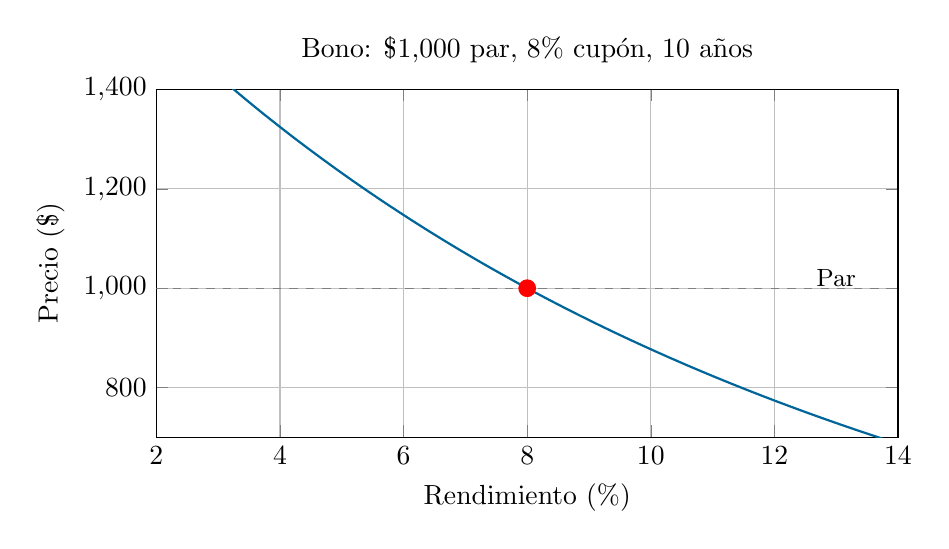
\begin{tikzpicture}
            \begin{axis}[
                xlabel={Rendimiento (\%)},
                ylabel={Precio (\$)},
                xmin=2, xmax=14,
                ymin=700, ymax=1400,
                grid=major,
                width=11cm,
                height=6cm,
                title={Bono: \$1,000 par, 8\% cupón, 10 años}
            ]
            \addplot[color=primaryblue, thick, domain=2:14, samples=50]
                {80*(1-(1+x/100)^(-10))/(x/100) + 1000*(1+x/100)^(-10)};

            % Línea de par
            \addplot[color=gray, dashed] coordinates {(2,1000) (14,1000)};
            \node at (axis cs:13,1020) {\small Par};

            % Punto de par
            \addplot[only marks, mark=*, mark size=3pt, color=red] coordinates {(8,1000)};
            \end{axis}
        \end{tikzpicture}
    \end{center}

    \textbf{Relación inversa:} Cuando el rendimiento sube, el precio baja (y viceversa).
\end{frame>

% ===========================================
% SECCIÓN 4: RENDIMIENTO AL VENCIMIENTO (YTM)
% ===========================================
\section{Rendimiento al Vencimiento (YTM)}

\begin{frame}{¿Qué es el YTM?}
    \begin{block}{Definición}
        El \textbf{Yield to Maturity (YTM)} es la tasa interna de retorno de un bono; es decir, la tasa que hace que el VP de los flujos futuros iguale el precio actual.
    \end{block}

    \pause
    \vspace{0.3cm}

    Matemáticamente, es la $r$ que resuelve:
    \[
    P = C \cdot \frac{1-(1+r)^{-n}}{r} + \frac{F}{(1+r)^n}
    \]

    \pause
    \vspace{0.3cm}

    \begin{alertblock}{Nota importante}
        El YTM no tiene solución algebraica directa. Se calcula por:
        \begin{itemize}
            \item Prueba y error / interpolación
            \item Calculadora financiera
            \item Métodos numéricos (Newton-Raphson)
        \end{itemize}
    \end{alertblock}
\end{frame}

\begin{frame}{Ejemplo: Calcular YTM}
    \begin{block}{Problema}
        Un bono con valor nominal \$1,000 y cupón 6\% anual se vende a \$950. Vence en 4 años. ¿Cuál es el YTM?
    \end{block}

    \pause
    \vspace{0.3cm}

    Buscamos $r$ tal que:
    \[
    950 = 60 \cdot \frac{1-(1+r)^{-4}}{r} + \frac{1,000}{(1+r)^4}
    \]

    \pause
    \textbf{Probando valores:}
    \begin{itemize}
        \item $r = 6\%$: $P = 1,000$ (muy alto)
        \item $r = 8\%$: $P = 933.76$ (muy bajo)
        \item $r = 7\%$: $P = 966.13$ (alto)
        \item $r = 7.5\%$: $P = 949.76 \approx 950$ \checkmark
    \end{itemize}

    \pause
    \textbf{YTM $\approx$ 7.5\%}
\end{frame>

\begin{frame}{Aproximación del YTM}
    \begin{alertblock}{Fórmula Aproximada}
        \[
        \boxed{YTM \approx \frac{C + \frac{F - P}{n}}{\frac{F + P}{2}}}
        \]
    \end{alertblock}

    \pause
    \vspace{0.3cm}

    \textbf{Ejemplo anterior:}
    \begin{align*}
        YTM &\approx \frac{60 + \frac{1000 - 950}{4}}{\frac{1000 + 950}{2}} \\[0.2cm]
        &= \frac{60 + 12.5}{975} = \frac{72.5}{975} = 7.44\%
    \end{align*}

    \pause
    Exacto: 7.5\%. La aproximación es razonablemente precisa.
\end{frame}

% ===========================================
% SECCIÓN 5: CURVA DE RENDIMIENTOS
% ===========================================
\section{Estructura Intertemporal de Tasas}

\begin{frame}{La Curva de Rendimientos (Yield Curve)}
    \begin{block}{Definición}
        La \textbf{curva de rendimientos} muestra la relación entre el plazo al vencimiento y el rendimiento de bonos de la misma calidad crediticia.
    \end{block}

    \pause
    \vspace{0.3cm}

    \begin{center}
        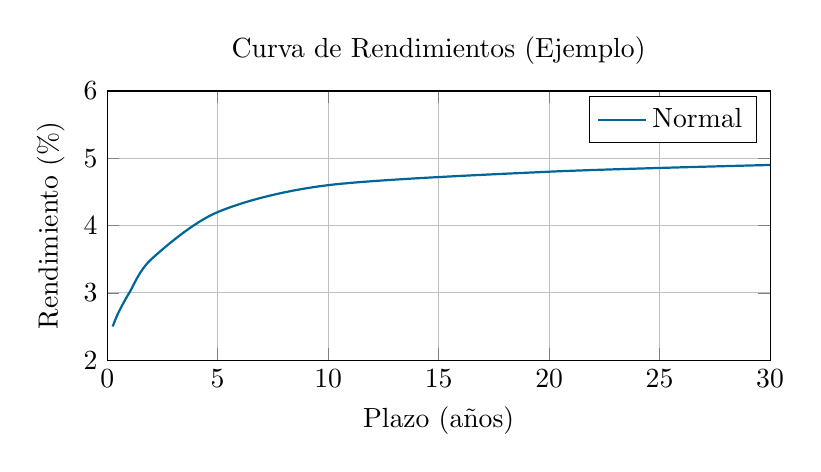
\begin{tikzpicture}
            \begin{axis}[
                xlabel={Plazo (años)},
                ylabel={Rendimiento (\%)},
                xmin=0, xmax=30,
                ymin=2, ymax=6,
                grid=major,
                width=10cm,
                height=5cm,
                title={Curva de Rendimientos (Ejemplo)}
            ]
            % Curva normal
            \addplot[color=primaryblue, thick, smooth] coordinates
                {(0.25,2.5) (0.5,2.7) (1,3.0) (2,3.5) (5,4.2) (10,4.6) (20,4.8) (30,4.9)};
            \addlegendentry{Normal}
            \end{axis}
        \end{tikzpicture}
    \end{center}
\end{frame}

\begin{frame}{Formas de la Curva}
    \begin{columns}
        \begin{column}{0.48\textwidth}
            \textbf{Normal (Pendiente Positiva)}

            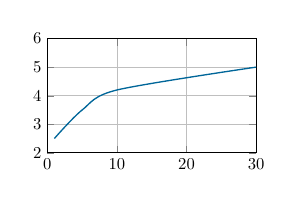
\begin{tikzpicture}[scale=0.6]
                \begin{axis}[
                    xmin=0, xmax=30, ymin=2, ymax=6,
                    width=6cm, height=4cm, grid=major
                ]
                \addplot[color=primaryblue, thick, smooth] coordinates
                    {(1,2.5) (5,3.5) (10,4.2) (30,5.0)};
                \end{axis}
            \end{tikzpicture}

            Tasas de largo plazo > corto plazo.

            \textit{Expectativa de crecimiento económico.}
        \end{column}

        \begin{column}{0.48\textwidth}
            \textbf{Invertida (Pendiente Negativa)}

            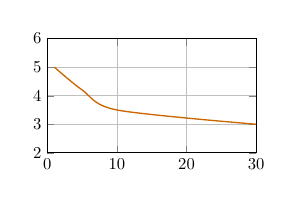
\begin{tikzpicture}[scale=0.6]
                \begin{axis}[
                    xmin=0, xmax=30, ymin=2, ymax=6,
                    width=6cm, height=4cm, grid=major
                ]
                \addplot[color=accentorange, thick, smooth] coordinates
                    {(1,5.0) (5,4.2) (10,3.5) (30,3.0)};
                \end{axis}
            \end{tikzpicture}

            Tasas de largo plazo < corto plazo.

            \textit{Señal histórica de recesión.}
        \end{column}
    \end{columns}

    \pause
    \vspace{0.5cm}

    \begin{alertblock}{Interpretación}
        La forma de la curva refleja expectativas del mercado sobre tasas futuras, inflación y crecimiento económico.
    \end{alertblock}
\end{frame}

\begin{frame}{Tasas Spot vs. Forward}
    \begin{block}{Tasa Spot ($s_t$)}
        Tasa de interés para un instrumento que comienza hoy y vence en $t$ períodos. Es la tasa ``del mercado'' para cada plazo.
    \end{block}

    \pause

    \begin{block}{Tasa Forward ($f_{t_1,t_2}$)}
        Tasa implícita para un período futuro, derivada de las tasas spot.

        La tasa forward del año 1 al año 2:
        \[
        (1 + s_2)^2 = (1 + s_1)(1 + f_{1,2})
        \]
    \end{block}

    \pause
    \vspace{0.3cm}

    \begin{exampleblock}{Ejemplo}
        Si $s_1 = 4\%$ y $s_2 = 5\%$:

        $f_{1,2} = \frac{(1.05)^2}{1.04} - 1 = \frac{1.1025}{1.04} - 1 = 6.01\%$
    \end{exampleblock}
\end{frame}

\section{Interpolación de Tasas}

\begin{frame}{Interpolación Lineal}
    \begin{block}{Problema}
        La curva de rendimientos da tasas para plazos específicos. ¿Qué tasa usar para un plazo intermedio?
    \end{block}

    \pause
    \vspace{0.3cm}

    \begin{block}{Interpolación Lineal}
        Si conocemos $r_1$ para plazo $t_1$ y $r_2$ para plazo $t_2$, la tasa para $t$ intermedio:
        \[
        \boxed{r_t = r_1 + \frac{(r_2 - r_1)(t - t_1)}{t_2 - t_1}}
        \]
    \end{block}

    \pause
    \vspace{0.3cm}

    \begin{exampleblock}{Ejemplo}
        Tasa a 2 años: 4\%. Tasa a 5 años: 5.5\%. ¿Tasa a 3 años?

        $r_3 = 4\% + \frac{(5.5\% - 4\%)(3 - 2)}{5 - 2} = 4\% + \frac{1.5\%}{3} = 4.5\%$
    \end{exampleblock>
\end{frame}

\begin{frame}{Interpolación: Ejemplo Visual}
    \begin{center}
        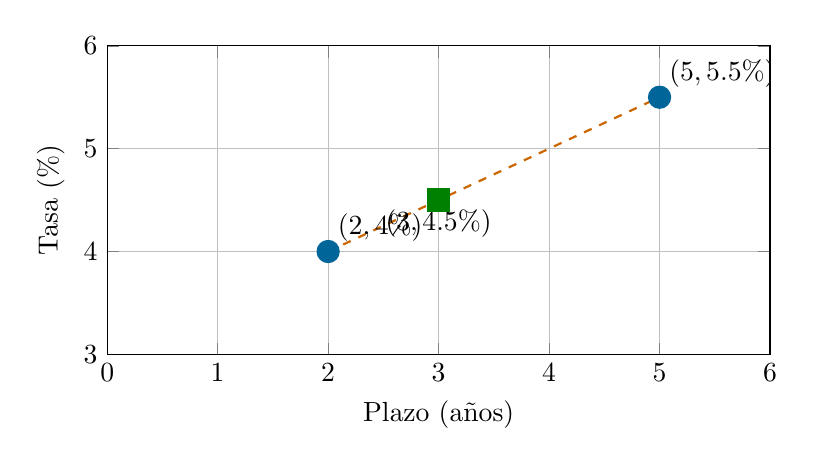
\begin{tikzpicture}
            \begin{axis}[
                xlabel={Plazo (años)},
                ylabel={Tasa (\%)},
                xmin=0, xmax=6,
                ymin=3, ymax=6,
                grid=major,
                width=10cm,
                height=5.5cm
            ]
            % Puntos conocidos
            \addplot[only marks, mark=*, mark size=4pt, color=primaryblue] coordinates {(2,4) (5,5.5)};

            % Línea de interpolación
            \addplot[color=accentorange, thick, dashed] coordinates {(2,4) (5,5.5)};

            % Punto interpolado
            \addplot[only marks, mark=square*, mark size=4pt, color=accentgreen] coordinates {(3,4.5)};

            % Etiquetas
            \node[above right] at (axis cs:2,4) {$(2, 4\%)$};
            \node[above right] at (axis cs:5,5.5) {$(5, 5.5\%)$};
            \node[below] at (axis cs:3,4.5) {$(3, 4.5\%)$};
            \end{axis}
        \end{tikzpicture}
    \end{center}

    La interpolación lineal asume que la tasa cambia uniformemente entre puntos conocidos.
\end{frame}

% ===========================================
% SECCIÓN 6: INTERPRETACIÓN VISUAL
% ===========================================
\section{Interpretación Visual}

\begin{frame}{Sensibilidad del Precio al Plazo}
    \begin{center}
        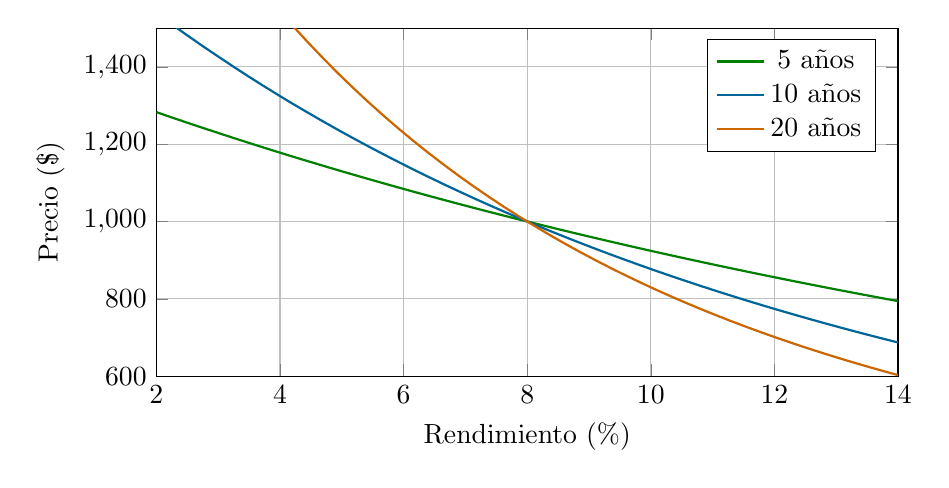
\begin{tikzpicture}
            \begin{axis}[
                xlabel={Rendimiento (\%)},
                ylabel={Precio (\$)},
                xmin=2, xmax=14,
                ymin=600, ymax=1500,
                grid=major,
                width=11cm,
                height=6cm,
                legend pos=north east
            ]
            % Bono 5 años
            \addplot[color=accentgreen, thick, domain=2:14, samples=50]
                {80*(1-(1+x/100)^(-5))/(x/100) + 1000*(1+x/100)^(-5)};
            \addlegendentry{5 años}

            % Bono 10 años
            \addplot[color=primaryblue, thick, domain=2:14, samples=50]
                {80*(1-(1+x/100)^(-10))/(x/100) + 1000*(1+x/100)^(-10)};
            \addlegendentry{10 años}

            % Bono 20 años
            \addplot[color=accentorange, thick, domain=2:14, samples=50]
                {80*(1-(1+x/100)^(-20))/(x/100) + 1000*(1+x/100)^(-20)};
            \addlegendentry{20 años}
            \end{axis}
        \end{tikzpicture}
    \end{center}

    \textbf{Observación:} Bonos de mayor plazo son más sensibles a cambios en tasas.
\end{frame}

\begin{frame}{Convergencia al Par}
    \begin{center}
        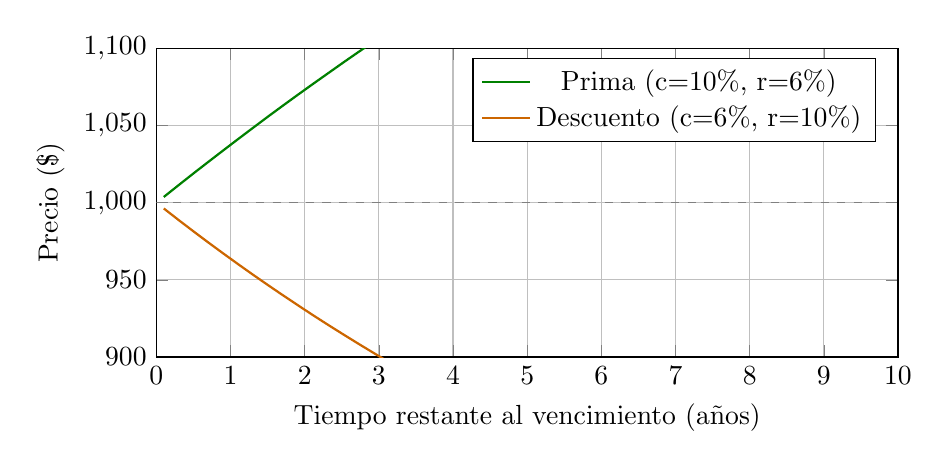
\begin{tikzpicture}
            \begin{axis}[
                xlabel={Tiempo restante al vencimiento (años)},
                ylabel={Precio (\$)},
                xmin=0, xmax=10,
                ymin=900, ymax=1100,
                grid=major,
                width=11cm,
                height=5.5cm,
                legend pos=north east
            ]
            % Bono prima (cupón > YTM)
            \addplot[color=accentgreen, thick, domain=0.1:10, samples=50]
                {100*(1-(1+0.06)^(-x))/(0.06) + 1000*(1+0.06)^(-x)};
            \addlegendentry{Prima (c=10\%, r=6\%)}

            % Bono descuento (cupón < YTM)
            \addplot[color=accentorange, thick, domain=0.1:10, samples=50]
                {60*(1-(1+0.10)^(-x))/(0.10) + 1000*(1+0.10)^(-x)};
            \addlegendentry{Descuento (c=6\%, r=10\%)}

            % Línea de par
            \addplot[color=gray, dashed] coordinates {(0,1000) (10,1000)};
            \end{axis}
        \end{tikzpicture}
    \end{center}

    Los bonos convergen al valor par conforme se acercan al vencimiento.
\end{frame}

% ===========================================
% SECCIÓN 7: TRUCOS Y HP 12C
% ===========================================
\section{Trucos de Estimación Mental}

\begin{frame}{Estimación Rápida del Cambio de Precio}
    \begin{alertblock}{Regla del 1\%}
        Para un bono con duración $D$ años:

        Si la tasa cambia $\Delta r$, el precio cambia aproximadamente:
        \[
        \Delta P \approx -D \times \Delta r \times P
        \]
    \end{alertblock}

    \pause
    \vspace{0.3cm}

    \textbf{Ejemplo simplificado:}

    Bono de 10 años (duración $\approx$ 7-8 años), precio \$1,000.

    Si las tasas suben 1\%:

    $\Delta P \approx -7.5 \times 0.01 \times 1000 = -\$75$

    Nuevo precio $\approx$ \$925.

    \pause
    \vspace{0.3cm}

    \textit{Nota: La ``duración'' precisa se verá en cursos avanzados.}
\end{frame}

\begin{frame}{Aproximación del YTM}
    \begin{alertblock}{Recordatorio de la fórmula aproximada}
        \[
        YTM \approx \frac{C + \frac{F - P}{n}}{\frac{F + P}{2}} = \frac{\text{Ingreso anual promedio}}{\text{Inversión promedio}}
        \]
    \end{alertblock}

    \pause
    \vspace{0.3cm}

    \textbf{Componentes:}
    \begin{itemize}
        \item Numerador: Cupón + amortización anual del descuento (o descuento de la prima)
        \item Denominador: Promedio entre precio pagado y valor a recibir
    \end{itemize}
\end{frame}

\section{Calculadora HP 12C}

\begin{frame}{HP 12C: Precio del Bono}
    \begin{block}{Problema}
        Bono: \$1,000 par, 7\% cupón semestral, 8 años, rendimiento requerido 9\%. ¿Precio?
    \end{block}

    \pause
    \vspace{0.2cm}

    \begin{center}
    \scriptsize
    \begin{tabular}{@{}lll@{}}
        \toprule
        \textbf{Teclas} & \textbf{Display} & \textbf{Descripción} \\
        \midrule
        \texttt{f CLX} & 0.00 & Limpiar \\
        \texttt{1000 FV} & 1,000.00 & Valor nominal \\
        \texttt{16 n} & 16.00 & 8 años $\times$ 2 = 16 semestres \\
        \texttt{4.5 i} & 4.50 & 9\%/2 = 4.5\% semestral \\
        \texttt{35 PMT} & 35.00 & Cupón = 1000 $\times$ 7\%/2 \\
        \texttt{PV} & \textbf{-889.30} & Precio del bono \\
        \bottomrule
    \end{tabular}
    \end{center}

    \pause
    \textbf{Precio = \$889.30} (descuento, porque YTM > cupón)
\end{frame}

\begin{frame}{HP 12C: Calcular YTM}
    \begin{block}{Problema}
        Mismo bono se vende a \$950. ¿Cuál es el YTM?
    \end{block}

    \pause
    \vspace{0.2cm}

    \begin{center}
    \scriptsize
    \begin{tabular}{@{}lll@{}}
        \toprule
        \textbf{Teclas} & \textbf{Display} & \textbf{Descripción} \\
        \midrule
        \texttt{f CLX} & 0.00 & Limpiar \\
        \texttt{950 CHS PV} & -950.00 & Precio (lo que pagas) \\
        \texttt{1000 FV} & 1,000.00 & Valor nominal \\
        \texttt{16 n} & 16.00 & 16 semestres \\
        \texttt{35 PMT} & 35.00 & Cupón semestral \\
        \texttt{i} & \textbf{3.97} & Tasa semestral \\
        \bottomrule
    \end{tabular}
    \end{center}

    \pause
    \textbf{YTM anual = $3.97\% \times 2 = 7.94\%$}

    (O efectiva: $(1.0397)^2 - 1 = 8.10\%$)
\end{frame}

% ===========================================
% SECCIÓN 8: EJERCICIOS PRÁCTICOS
% ===========================================
\section{Ejercicios Prácticos}

\begin{frame}{Ejercicio 1: Precio del Bono}
    \begin{block}{Problema}
        Un bono del gobierno tiene valor nominal \$10,000, cupón 5\% anual, vence en 6 años. Si el rendimiento requerido es 4\%, ¿cuál es el precio?
    \end{block}

    \pause
    \vspace{0.3cm}

    \textbf{Datos:} $F = 10,000$, $C = 500$, $n = 6$, $r = 4\%$

    \textbf{Solución:}
    \begin{align*}
        P &= 500 \cdot \frac{1-(1.04)^{-6}}{0.04} + \frac{10,000}{(1.04)^6} \\[0.2cm]
        P &= 500 \times 5.2421 + 10,000 \times 0.7903 \\[0.2cm]
        P &= 2,621.05 + 7,903.15 = \$10,524.20
    \end{align*}

    \pause
    El bono se vende con \textbf{prima} porque cupón (5\%) > rendimiento (4\%).
\end{frame}

\begin{frame}{Ejercicio 2: YTM con Fórmula Aproximada}
    \begin{block}{Problema}
        Un bono con valor par \$1,000, cupón 9\%, vence en 12 años y se vende a \$1,080. Estima el YTM.
    \end{block}

    \pause
    \vspace{0.3cm}

    \textbf{Usando la aproximación:}
    \begin{align*}
        YTM &\approx \frac{C + \frac{F - P}{n}}{\frac{F + P}{2}} \\[0.2cm]
        YTM &\approx \frac{90 + \frac{1000 - 1080}{12}}{\frac{1000 + 1080}{2}} \\[0.2cm]
        YTM &\approx \frac{90 - 6.67}{1040} = \frac{83.33}{1040} = 8.01\%
    \end{align*}

    \pause
    El YTM es menor que el cupón porque el bono está en prima.
\end{frame}

\begin{frame}{Ejercicio 3: Interpolación de Tasas}
    \begin{block}{Problema}
        La curva de rendimientos muestra:
        \begin{itemize}
            \item 1 año: 3.5\%
            \item 3 años: 4.2\%
            \item 5 años: 4.8\%
            \item 10 años: 5.5\%
        \end{itemize}
        ¿Cuál es la tasa para un bono a 7 años?
    \end{block}

    \pause
    \vspace{0.3cm}

    \textbf{Interpolando entre 5 y 10 años:}
    \begin{align*}
        r_7 &= 4.8\% + \frac{(5.5\% - 4.8\%)(7 - 5)}{10 - 5} \\[0.2cm]
        r_7 &= 4.8\% + \frac{0.7\% \times 2}{5} = 4.8\% + 0.28\% = 5.08\%
    \end{align*}
\end{frame}

\begin{frame}{Ejercicio 4: Bono Cupón Cero}
    \begin{block}{Problema}
        Un bono cupón cero (sin pagos periódicos) con valor nominal \$1,000 vence en 5 años. Si el rendimiento requerido es 6\%, ¿cuál es el precio?
    \end{block}

    \pause
    \vspace{0.3cm}

    \textbf{Sin cupones, solo el principal:}
    \begin{align*}
        P &= \frac{F}{(1+r)^n} = \frac{1,000}{(1.06)^5} \\[0.2cm]
        P &= \frac{1,000}{1.3382} = \$747.26
    \end{align*}

    \pause
    \vspace{0.3cm}

    \begin{exampleblock}{Observación}
        Los bonos cupón cero siempre se venden con descuento (salvo tasas negativas).
    \end{exampleblock>
\end{frame}

\begin{frame}{Ejercicio 5: Comparar Bonos}
    \begin{block}{Problema}
        Bono A: cupón 8\%, 10 años, precio \$950.

        Bono B: cupón 6\%, 10 años, precio \$900.

        ¿Cuál tiene mayor YTM?
    \end{block}

    \pause
    \vspace{0.2cm}

    \textbf{Aproximación para Bono A:}
    $YTM_A \approx \frac{80 + (1000-950)/10}{975} = \frac{85}{975} = 8.72\%$

    \pause
    \textbf{Aproximación para Bono B:}
    $YTM_B \approx \frac{60 + (1000-900)/10}{950} = \frac{70}{950} = 7.37\%$

    \pause
    \vspace{0.3cm}

    \textbf{Respuesta:} Bono A tiene mayor YTM (8.72\% vs 7.37\%).
\end{frame}

% ===========================================
% SECCIÓN 9: PYTHON
% ===========================================
\section{Python con numpy-financial}

\begin{frame}[fragile]{Python: Precio del Bono}
    \begin{lstlisting}[style=pythonstyle]
import numpy_financial as npf

def precio_bono(F, c, n, r, m=1):
    """
    F: Valor nominal
    c: Tasa cupon anual
    n: Anos al vencimiento
    r: Rendimiento requerido anual
    m: Pagos por ano (1=anual, 2=semestral)
    """
    C = F * c / m      # Cupon por periodo
    r_per = r / m      # Tasa por periodo
    n_per = n * m      # Numero de periodos

    # PV = VP cupones + VP principal
    pv_cupones = npf.pv(r_per, n_per, -C, 0)
    pv_principal = F / (1 + r_per)**n_per

    return pv_cupones + pv_principal

# Ejemplo
precio = precio_bono(F=1000, c=0.08, n=10, r=0.10)
print(f"Precio del bono: ${precio:,.2f}")
    \end{lstlisting}
\end{frame>

\begin{frame}[fragile]{Python: Calcular YTM}
    \begin{lstlisting}[style=pythonstyle]
import numpy_financial as npf

def ytm_bono(precio, F, c, n, m=1):
    """Calcula YTM usando numpy-financial."""
    C = F * c / m
    n_per = n * m

    # Construir flujos: -precio, cupones, ultimo cupon + principal
    flujos = [-precio] + [C]*(n_per-1) + [C + F]

    # IRR da tasa por periodo
    irr_per = npf.irr(flujos)

    # Convertir a anual
    ytm_anual = irr_per * m  # Nominal
    ytm_efectivo = (1 + irr_per)**m - 1  # Efectivo

    return ytm_anual, ytm_efectivo

# Ejemplo
ytm_nom, ytm_ef = ytm_bono(precio=950, F=1000, c=0.07, n=8, m=2)
print(f"YTM nominal: {ytm_nom*100:.2f}%")
print(f"YTM efectivo: {ytm_ef*100:.2f}%")
    \end{lstlisting}
\end{frame}

\begin{frame}[fragile]{Python: Curva de Rendimientos}
    \begin{lstlisting}[style=pythonstyle]
import matplotlib.pyplot as plt
import numpy as np

# Datos de la curva
plazos = [0.25, 0.5, 1, 2, 5, 10, 20, 30]
tasas = [2.5, 2.7, 3.0, 3.5, 4.2, 4.6, 4.8, 4.9]

# Interpolacion para puntos intermedios
from scipy import interpolate
f = interpolate.interp1d(plazos, tasas, kind='linear')
plazos_interp = np.linspace(0.25, 30, 100)
tasas_interp = f(plazos_interp)

plt.figure(figsize=(10, 5))
plt.plot(plazos_interp, tasas_interp, 'b-', label='Curva interpolada')
plt.scatter(plazos, tasas, color='red', s=50, label='Datos')
plt.xlabel('Plazo (anos)')
plt.ylabel('Rendimiento (%)')
plt.title('Curva de Rendimientos')
plt.legend(); plt.grid(True)
    \end{lstlisting}
\end{frame}

% ===========================================
% SECCIÓN 10: RESUMEN Y TAREA
% ===========================================
\section{Resumen y Tarea}

\begin{frame}{Resumen de Fórmulas}
    \textbf{Precio del Bono:}
    \[
    P = C \cdot \frac{1-(1+r)^{-n}}{r} + \frac{F}{(1+r)^n}
    \]

    \textbf{YTM Aproximado:}
    \[
    YTM \approx \frac{C + (F-P)/n}{(F+P)/2}
    \]

    \textbf{Interpolación Lineal:}
    \[
    r_t = r_1 + \frac{(r_2 - r_1)(t - t_1)}{t_2 - t_1}
    \]

    \textbf{Clasificación:}
    Prima: $P > F$ | Par: $P = F$ | Descuento: $P < F$
\end{frame}

\begin{frame}{Conceptos Clave}
    \begin{enumerate}
        \item El \textbf{precio} de un bono es el VP de cupones + VP del principal
        \item \textbf{YTM} es la TIR del bono (rendimiento si se mantiene hasta vencimiento)
        \item Relación \textbf{inversa} entre precio y rendimiento
        \item La \textbf{curva de rendimientos} muestra tasas por plazo
        \item \textbf{Interpolación} para obtener tasas de plazos intermedios
        \item Bonos de mayor plazo son más \textbf{sensibles} a cambios de tasas
        \item Los precios convergen al \textbf{par} al acercarse al vencimiento
    \end{enumerate}
\end{frame}

\begin{frame}{Tarea para la Próxima Sesión}
    \begin{enumerate}
        \item \textbf{HP 12C:} Calcular precio y YTM de un bono con cupón 6\% semestral, 5 años, valor par \$1,000, rendimiento 8\%.

        \vspace{0.3cm}

        \item \textbf{Interpolación:} Dada la curva (1 año: 4\%, 5 años: 5.5\%, 10 años: 6.2\%), encuentra la tasa a 3 y 7 años.

        \vspace{0.3cm}

        \item \textbf{Análisis:} Un bono cupón 10\% se vende a \$1,100. ¿El YTM es mayor o menor que 10\%? Explica sin calcular.

        \vspace{0.3cm}

        \item \textbf{Python:} Grafica cómo cambia el precio de un bono (8\% cupón, 15 años) cuando el YTM varía de 2\% a 14\%.
    \end{enumerate}
\end{frame}

% ===========================================
% CIERRE
% ===========================================

\begin{frame}
    \begin{center}
        \Huge \textcolor{primaryblue}{\textbf{¿Preguntas?}}

        \vspace{1cm}
        \Large Próxima Sesión:\\
        \textbf{VPN y TIR}

        \vspace{0.5cm}
        \normalsize Semana 5, Clase 1
    \end{center}
\end{frame}

\end{document}
